\documentclass{standalone}
\usepackage{tikz}
\usepackage{qcircuit}
\usepackage{braket}

\begin{document}
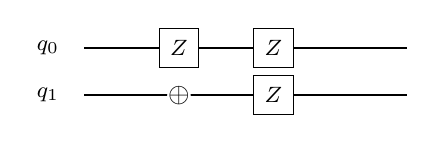
\begin{tikzpicture}[
  wire/.style={thick}]
  \draw[wire] (0,-0.00) -- (4.10,-0.00);
  \node[font=\footnotesize, anchor=east] at (-0.2,-0.00) {$q_{0}$};
  \draw[wire] (0,-0.60) -- (4.10,-0.60);
  \node[font=\footnotesize, anchor=east] at (-0.2,-0.60) {$q_{1}$};
  \node[draw, minimum size=0.5cm, fill=white, font=\footnotesize] at (1.20,-0.00) {$Z$};
  \node[circle, fill=white, minimum size=3.0mm, inner sep=0pt] at (1.20,-0.60) {};
  \node at (1.20,-0.60) {$\oplus$};
  \node[draw, minimum size=0.5cm, fill=white, font=\footnotesize] at (2.40,-0.00) {$Z$};
  \node[draw, minimum size=0.5cm, fill=white, font=\footnotesize] at (2.40,-0.60) {$Z$};
\end{tikzpicture}
\end{document}
